\documentclass[10pt,oneside]{article}
\usepackage{hla2025}
\NeedsTeXFormat{LaTeX2e}
\ProvidesFile{rl-graphics.sty}[2026/08/24 v0.3 Requirements Lab family graphics]

% Adapted from the supplied HLA Requirements Lab family-graphics source. The
% adapter deliberately keeps graphics-only colors and macros separate from
% readable document text so orange remains an accent rather than a text color.
\RequirePackage{etoolbox}
\usetikzlibrary{arrows.meta,calc,positioning,backgrounds,shapes.geometric}

\definecolor{RLGraphInk}{HTML}{172334}
\definecolor{RLGraphMuted}{HTML}{687386}
\definecolor{RLGraphRule}{HTML}{D6DEE8}
\definecolor{RLGraphWhite}{HTML}{FFFFFF}
\definecolor{RLGraphFramework}{HTML}{496B91}
\definecolor{RLGraphFrameworkTint}{HTML}{EAF0F6}
\definecolor{RLGraphInterface}{HTML}{6D5FA6}
\definecolor{RLGraphInterfaceTint}{HTML}{EEEAF7}
\definecolor{RLGraphOMT}{HTML}{CF7B31}
\definecolor{RLGraphOMTTint}{HTML}{F7EEE4}
\definecolor{RLGraph2010}{HTML}{637489}
\definecolor{RLGraph2010Tint}{HTML}{EBEFF4}
\definecolor{RLGraph2025}{HTML}{E7773F}
\definecolor{RLGraph2025Tint}{HTML}{F7E8DF}

\def\RLGraphFrameworkFamily{framework}
\def\RLGraphInterfaceFamily{interface}
\def\RLGraphOmtFamily{omt}

\newcommand{\RLSetGraphicFamily}[1]{%
    \edef\RLGraphFamilyValue{#1}%
    \ifx\RLGraphFamilyValue\RLGraphFrameworkFamily
        \colorlet{RLGraphAccent}{RLGraphFramework}%
        \colorlet{RLGraphAccentTint}{RLGraphFrameworkTint}%
    \fi
    \ifx\RLGraphFamilyValue\RLGraphInterfaceFamily
        \colorlet{RLGraphAccent}{RLGraphInterface}%
        \colorlet{RLGraphAccentTint}{RLGraphInterfaceTint}%
    \fi
    \ifx\RLGraphFamilyValue\RLGraphOmtFamily
        \colorlet{RLGraphAccent}{RLGraphOMT}%
        \colorlet{RLGraphAccentTint}{RLGraphOMTTint}%
    \fi
}

\newcommand{\RLSetGraphicEdition}[1]{%
    \ifnum#1=2010\relax
        \colorlet{RLGraphEdition}{RLGraph2010}%
        \colorlet{RLGraphEditionTint}{RLGraph2010Tint}%
    \else
        \colorlet{RLGraphEdition}{RLGraph2025}%
        \colorlet{RLGraphEditionTint}{RLGraph2025Tint}%
    \fi
}

\tikzset{
    rl graph line/.style={draw=RLGraphAccent,line width=1.15pt,line cap=round,line join=round},
    rl graph fine/.style={draw=RLGraphAccent!55,line width=0.62pt,line cap=round,line join=round},
    rl graph faint/.style={draw=RLGraphAccent!25,line width=0.48pt,line cap=round,line join=round},
    rl graph node/.style={circle,fill=RLGraphAccent,draw=RLGraphWhite,line width=0.7pt,minimum size=4.1pt,inner sep=0pt},
    rl graph node open/.style={circle,fill=RLGraphWhite,draw=RLGraphAccent,line width=0.85pt,minimum size=4.1pt,inner sep=0pt},
    rl graph arrow/.style={draw=RLGraphAccent,line width=1.0pt,-{Stealth[length=4.2pt,width=3.6pt]},line cap=round},
    rl graph arrow muted/.style={draw=RLGraphAccent!55,line width=0.78pt,-{Stealth[length=3.7pt,width=3.1pt]},line cap=round},
}

\newcommand{\RLGraphicEditionFrame}[1]{%
    \ifnum#1=2010\relax
        \draw[draw=RLGraphAccent!45,line width=0.82pt] (-1.55,-1.55) rectangle (1.55,1.55);
        \draw[draw=RLGraphAccent!16,line width=0.55pt] (-1.35,-1.35) rectangle (1.35,1.35);
    \else
        \draw[draw=RLGraphAccent!34,line width=0.74pt] (-1.55,-1.38) rectangle (1.34,1.50);
        \draw[draw=RLGraphAccent!18,line width=0.58pt] (-1.18,-1.60) rectangle (1.60,1.18);
        \draw[draw=RLGraphEdition,line width=1.05pt] (1.34,0.54) -- (1.34,1.50) -- (0.42,1.50);
    \fi
}

\newcommand{\RLGraphCube}[4]{%
    \begin{scope}[shift={(#1,#2)},scale=#3]
        \coordinate (rla) at (-0.72,-0.62);
        \coordinate (rlb) at (0.72,-0.62);
        \coordinate (rlc) at (0.72,0.82);
        \coordinate (rld) at (-0.72,0.82);
        \coordinate (rlap) at (-0.20,-0.28);
        \coordinate (rlbp) at (1.24,-0.28);
        \coordinate (rlcp) at (1.24,1.16);
        \coordinate (rldp) at (-0.20,1.16);
        \draw[draw=RLGraphAccent!#4,line width=0.78pt,line join=round] (rla)--(rlb)--(rlc)--(rld)--cycle;
        \draw[draw=RLGraphAccent!#4,line width=0.78pt,line join=round] (rlap)--(rlbp)--(rlcp)--(rldp)--cycle;
        \foreach \p/\q in {rla/rlap,rlb/rlbp,rlc/rlcp,rld/rldp}{\draw[draw=RLGraphAccent!#4,line width=0.78pt] (\p)--(\q);}
    \end{scope}
}

\newcommand{\RLOverviewGlyph}[1]{%
    \RLGraphicEditionFrame{#1}%
    \ifnum#1=2010\relax
        \draw[rl graph fine] (0,0) circle (1.02);
        \draw[rl graph faint] (0,0) circle (0.58);
        \coordinate (rln1) at (90:1.02);
        \coordinate (rln2) at (0:1.02);
        \coordinate (rln3) at (270:1.02);
        \coordinate (rln4) at (180:1.02);
        \foreach \n in {rln1,rln2,rln3,rln4}{\draw[rl graph fine] (0,0) -- (\n);}
        \draw[rl graph line] (rln1)--(rln2)--(rln3)--(rln4)--cycle;
        \node[rl graph node] at (0,0) {};
        \foreach \n in {rln1,rln2,rln3,rln4}{\node[rl graph node open] at (\n) {};}
    \else
        \draw[rl graph fine] (0,0) circle (0.84);
        \draw[rl graph faint] (0.12,-0.06) circle (1.18);
        \coordinate (rln1) at (104:1.18);
        \coordinate (rln2) at (38:1.18);
        \coordinate (rln3) at (-28:1.18);
        \coordinate (rln4) at (-104:1.18);
        \coordinate (rln5) at (176:1.18);
        \coordinate (rln6) at (1.72,0.48);
        \draw[rl graph fine] (rln1)--(rln2)--(rln3)--(rln4)--(rln5)--cycle;
        \draw[rl graph line] (rln1)--(0.08,0.10)--(rln3);
        \draw[rl graph line] (rln5)--(0.08,0.10)--(rln2);
        \draw[rl graph fine] (rln4)--(0.08,0.10);
        \draw[draw=RLGraphEdition,line width=1.22pt,line cap=round] (0.08,0.10)--(rln6);
        \node[rl graph node] at (0.08,0.10) {};
        \foreach \n in {rln1,rln2,rln3,rln4,rln5}{\node[rl graph node open] at (\n) {};}
        \node[circle,fill=RLGraphEdition,draw=RLGraphWhite,line width=0.7pt,minimum size=4.5pt,inner sep=0pt] at (rln6) {};
    \fi
}

\newcommand{\RLInterfaceGlyph}[1]{%
    \RLGraphicEditionFrame{#1}%
    \ifnum#1=2010\relax
        \draw[rl graph line,rounded corners=2pt] (-1.27,-0.56) rectangle (-0.62,0.56);
        \draw[rl graph line,rounded corners=2pt] (0.62,-0.56) rectangle (1.27,0.56);
        \draw[rl graph fine] (-0.12,-0.82) rectangle (0.12,0.82);
        \foreach \y in {-0.26,0,0.26}{%
            \node[rl graph node open] at (-0.62,\y) {};
            \node[rl graph node open] at (0.62,\y) {};
        }
        \draw[rl graph arrow] (-0.52,0.22) -- (0.50,0.22);
        \draw[rl graph arrow] (0.52,-0.22) -- (-0.50,-0.22);
    \else
        \draw[rl graph fine,rounded corners=2pt] (-1.37,-0.72) rectangle (-0.62,0.48);
        \draw[rl graph line,rounded corners=2pt] (-1.22,-0.49) rectangle (-0.47,0.71);
        \draw[rl graph fine,rounded corners=2pt] (0.62,-0.48) rectangle (1.37,0.72);
        \draw[rl graph line,rounded corners=2pt] (0.47,-0.71) rectangle (1.22,0.49);
        \draw[rl graph fine] (-0.18,-0.90) -- (-0.18,0.90);
        \draw[rl graph fine] (0.18,-0.90) -- (0.18,0.90);
        \draw[rl graph arrow] (-0.40,0.42) -- (0.40,0.42);
        \draw[rl graph arrow muted] (0.40,0.00) -- (-0.40,0.00);
        \draw[rl graph arrow] (-0.40,-0.42) -- (0.40,-0.42);
        \draw[draw=RLGraphEdition,line width=1.05pt,-{Stealth[length=4.0pt,width=3.4pt]},line cap=round]
            (0.86,0.82) .. controls (0.20,1.22) and (-0.34,1.16) .. (-0.88,0.77);
        \node[diamond,fill=RLGraphWhite,draw=RLGraphAccent,line width=0.9pt,minimum size=8.5pt,inner sep=0pt] at (0,0) {};
    \fi
}

\newcommand{\RLOMTGlyph}[1]{%
    \RLGraphicEditionFrame{#1}%
    \ifnum#1=2010\relax
        \RLGraphCube{-0.22}{-0.18}{0.92}{70}
        \draw[rl graph fine] (-0.88,-0.20)--(-0.16,0.52)--(0.72,-0.12);
        \node[rl graph node] at (-0.88,-0.20) {};
        \node[rl graph node open] at (-0.16,0.52) {};
        \node[rl graph node] at (0.72,-0.12) {};
        \draw[rl graph faint] (-0.16,0.52)--(0.66,0.95);
        \node[rl graph node open] at (0.66,0.95) {};
    \else
        \RLGraphCube{-0.48}{-0.37}{0.80}{55}
        \RLGraphCube{0.08}{-0.04}{0.64}{28}
        \draw[rl graph line] (-0.98,-0.34)--(-0.30,0.38)--(0.54,-0.16)--(0.90,0.58);
        \draw[rl graph fine] (-0.30,0.38)--(0.20,0.92);
        \draw[draw=RLGraphEdition,line width=1.15pt,line cap=round] (0.90,0.58)--(1.52,0.88);
        \node[rl graph node] at (-0.98,-0.34) {};
        \node[rl graph node open] at (-0.30,0.38) {};
        \node[rl graph node] at (0.54,-0.16) {};
        \node[rl graph node open] at (0.90,0.58) {};
        \node[rl graph node open] at (0.20,0.92) {};
        \node[rectangle,fill=RLGraphEdition,draw=RLGraphWhite,line width=0.7pt,minimum size=5.2pt,inner sep=0pt] at (1.52,0.88) {};
    \fi
}

\newcommand{\RLFamilyGlyph}[2]{%
    % Product preambles pass the family as a named macro. Expand it before
    % comparing the volume so all six covers select their dedicated glyph.
    \edef\RLGraphFamily{#2}%
    \RLSetGraphicFamily{\RLGraphFamily}%
    \RLSetGraphicEdition{#1}%
    \ifx\RLGraphFamily\RLGraphFrameworkFamily\RLOverviewGlyph{#1}\fi
    \ifx\RLGraphFamily\RLGraphInterfaceFamily\RLInterfaceGlyph{#1}\fi
    \ifx\RLGraphFamily\RLGraphOmtFamily\RLOMTGlyph{#1}\fi
}

\NeedsTeXFormat{LaTeX2e}
\ProvidesFile{rl-code.sty}[2026/08/23 v0.1 Requirements Lab code and XML]

\RequirePackage{xcolor}
\RequirePackage{listings}

% Plain LaTeX's verbatim environment must appear directly in the document
% source, so the shared API supplies the surrounding typography as commands.
\newcommand{\RLCodeStart}{\par\smallskip\noindent\begingroup\small\RLMono\color{RLInk}}
\newcommand{\RLCodeEnd}{\endgroup\smallskip}

\newcommand{\RLCodeInline}[1]{\colorbox{RLCode}{\RLMono\fontsize{8.4pt}{10pt}\selectfont\ #1\ }}

\lstdefinestyle{RLCodeListing}{%
    basicstyle=\RLMono\fontsize{8.2pt}{10.4pt}\selectfont\color{RLInk},
    columns=fullflexible,
    keepspaces=true,
    showstringspaces=false,
    breaklines=false,
    frame=single,
    framerule=0.35pt,
    rulecolor=\color{RLLine},
    backgroundcolor=\color{RLCode},
    xleftmargin=6pt,
    xrightmargin=6pt,
    aboveskip=5pt,
    belowskip=6pt,
    captionpos=b
}
\lstnewenvironment{RLCodeBlock}{\lstset{style=RLCodeListing}}{}

\NeedsTeXFormat{LaTeX2e}
\ProvidesFile{rl-tables.sty}[2026/08/23 v0.1 Requirements Lab table taxonomy]

\RequirePackage{array}
\RequirePackage{booktabs}
\RequirePackage{colortbl}
\RequirePackage{longtable}
\RequirePackage{tabularx}
\RequirePackage{xparse}

\newcolumntype{Y}{>{\RaggedRight\arraybackslash}X}
\newcolumntype{L}[1]{>{\RaggedRight\arraybackslash}p{#1}}
\newcolumntype{C}[1]{>{\Centering\arraybackslash}p{#1}}
\newcommand{\RLTableHeader}[1]{\strut\RLSans\bfseries\color{RLBlueDeep}#1}
\newcommand{\RLTableHeaderCell}[1]{\RLTableHeader{#1}}
\newcommand{\RLTableHeaderBlock}[2]{%
    \parbox{#1}{\RLSans\bfseries\fontsize{7.8pt}{9.2pt}\selectfont\color{RLBlueDeep}#2}%
}
\newcommand{\RLTableGroupHeader}[1]{%
    {\RLSans\bfseries\fontsize{7.2pt}{8.5pt}\selectfont\addfontfeatures{LetterSpace=1.1}\color{RLBlue}\MakeUppercase{#1}}%
}
% The header band is a single colortbl row, matching the golden-master
% prototype rather than a collection of individually filled label chips.
\newcommand{\RLProductionHeaderBand}{\rowcolor{RLTableBand}}
\newcommand{\RLProductionHeaderSpace}{\addlinespace[1.5pt]}
\newcommand{\RLProductionTopRule}{\toprule[0.70pt]}
\newcommand{\RLProductionHeaderRule}{\midrule[0.45pt]}
\newcommand{\RLProductionRowRule}{\midrule[0.20pt]}
\newcommand{\RLProductionBottomRule}{\bottomrule[0.80pt]}
\newcommand{\RLTableCaption}[1]{%
    \par\vspace{4pt}\noindent
    {\RLSans\fontsize{7.4pt}{9pt}\selectfont\addfontfeatures{LetterSpace=1.2}\MakeUppercase{#1}}\par
    \vspace{5pt}
}
\newcommand{\RLInlineTableCaption}[2]{%
    \par\vspace{4pt}\noindent
    {\RLSans\fontsize{7.4pt}{9pt}\selectfont\addfontfeatures{LetterSpace=1.2}\MakeUppercase{TABLE~#1}}\hspace{6pt}%
    {\RLSans\bfseries\fontsize{9.3pt}{11.2pt}\selectfont #2}\par
    \vspace{5pt}
}

\NewDocumentEnvironment{RLReferenceTable}{m m +b}{%
    \RLTableCaption{#1}\phantomsection\label{#2}
        \begin{tabularx}{\linewidth}{@{}L{0.27\linewidth}Y@{}}
        \toprule
        \RLTableHeaderCell{Term} & \RLTableHeaderCell{Meaning} \\
        \midrule
        #3
        \bottomrule
        \end{tabularx}
}{ }

\NewDocumentEnvironment{RLRegistryTable}{m m +b}{%
    \RLTableCaption{#1}\phantomsection\label{#2}
        \begin{tabularx}{\linewidth}{@{}L{0.22\linewidth}L{0.24\linewidth}Y@{}}
        \toprule
        \RLTableHeaderCell{Identifier} & \RLTableHeaderCell{Category} & \RLTableHeaderCell{Description} \\
        \midrule
        #3
        \bottomrule
        \end{tabularx}
}{ }

\NewDocumentEnvironment{RLDenseTable}{m m m +b}{%
    \RLTableCaption{#1}\phantomsection\label{#2}
        \begin{longtable}{@{}#3@{}}
        \toprule
        #4
        \bottomrule
    \end{longtable}
}{ }

\NewDocumentEnvironment{RLLandscapeTable}{m m m +b}{%
    \begin{RLLandscapePage}
        \RLTableCaption{#1}\phantomsection\label{#2}
        \begin{longtable}{@{}#3@{}}
        #4
        \end{longtable}
    \end{RLLandscapePage}
}{ }

\newcommand{\RLContinuedHeader}[1]{\multicolumn{1}{l}{\RLSans\fontsize{7.8pt}{9.3pt}\selectfont\color{RLMid}#1}\tabularnewline}

\newcommand{\RLSerifScale}{0.82}
\NeedsTeXFormat{LaTeX2e}
\ProvidesFile{rl-publication.sty}[2026/08/24 v0.1 Requirements Lab HLA publication profile]

% High-level bridge used by all six HLA source compilations.  It maps the
% document-level HLA metadata used by the faithful body adapters into the
% shared Requirements Lab style profile.  The body adapters remain free to
% preserve edition-specific geometry; the visible style contract is shared.
% Legacy adapters load their source-faithful style first, so install the
% canonical reading faces here after that style has finished declaring its
% defaults.  The modern class has already loaded rl-type.sty.
\ifdefined\RLSerif\else
    \NeedsTeXFormat{LaTeX2e}
\ProvidesFile{rl-type.sty}[2026/08/23 v0.1 Requirements Lab typography]

\RequirePackage{fontspec}

\newfontfamily\RLSerif{Noto Serif}[Ligatures=NoCommon]
% Inter is the prototype sans face. The checked-in role files are static
% Regular, Italic, and ExtraBold instances generated from the official
% package, so XeLaTeX embeds the intended faces without engine-specific axis
% fallbacks.
\IfFileExists{../requirements-lab/fonts/Inter-Regular.ttf}{}{\PackageError{requirements-lab}{Inter font files are missing}{Restore the checked-in Requirements Lab font bundle before building.}}
\newfontfamily\RLSans{Inter}[
    Path=../requirements-lab/fonts/,
    UprightFont=Inter-Regular.ttf,
    ItalicFont=Inter-Italic.ttf,
    BoldFont=Inter-ExtraBold.ttf,
    BoldItalicFont=Inter-Italic.ttf,
    Ligatures=NoCommon]
\setsansfont{Inter}[
    Path=../requirements-lab/fonts/,
    UprightFont=Inter-Regular.ttf,
    ItalicFont=Inter-Italic.ttf,
    BoldFont=Inter-ExtraBold.ttf,
    BoldItalicFont=Inter-Italic.ttf,
    Ligatures=NoCommon]
\newfontfamily\RLMono{DejaVu Sans Mono}[Ligatures=NoCommon]

\setmainfont{Noto Serif}[Ligatures=NoCommon]

\newcommand{\RLBodyFont}{\RLSerif\fontsize{9.75pt}{13.25pt}\selectfont\color{RLInk}}
\newcommand{\RLTableFont}{\RLSans\fontsize{8.55pt}{10.7pt}\selectfont\color{RLInk}}
\newcommand{\RLSmallFont}{\RLSans\fontsize{8.25pt}{10.2pt}\selectfont\color{RLInk}}
\newcommand{\RLIdentifier}[1]{{\RLMono\fontsize{8.65pt}{10.7pt}\selectfont\color{RLBlueDeep}\mbox{#1}}}
\newcommand{\RLType}[1]{{\RLMono\fontsize{8.65pt}{10.7pt}\selectfont\color{RLBlueDeep}\mbox{#1}}}
\newcommand{\RLXML}[1]{{\RLMono\fontsize{8.5pt}{10.5pt}\selectfont\color{RLBlueDeep}\mbox{#1}}}
\newcommand{\RLValue}[1]{{\RLMono\fontsize{8.65pt}{10.7pt}\selectfont\color{RLInk}\mbox{#1}}}
\newcommand{\RLService}[1]{{\RLSans\fontsize{8.9pt}{11pt}\selectfont\color{RLBlueDeep}#1}}
\newcommand{\RLClass}[1]{\RLIdentifier{#1}}
\newcommand{\RLAttribute}[1]{\RLIdentifier{#1}}
\newcommand{\RLInteraction}[1]{\RLIdentifier{#1}}

\fi
\NeedsTeXFormat{LaTeX2e}
\ProvidesFile{rl-fixed-page.sty}[2026/08/24 v0.1 Requirements Lab fixed-page furniture]

% Shared page furniture for source-faithful fixed-coordinate adapters.  The
% adapter deliberately depends on the same Requirements Lab tokens as the
% natural-flow class, so a document can preserve its measured body geometry
% without inventing a second visual language.
\RequirePackage{etoolbox}
\RequirePackage{fancyhdr}
\RequirePackage{fontspec}
\RequirePackage{tikz}

\makeatletter
\@ifundefined{RLPublicationName}{\NeedsTeXFormat{LaTeX2e}
\ProvidesFile{rl-brand.sty}[2026/08/23 v0.1 Requirements Lab brand tokens]

\RequirePackage{xcolor}
\RequirePackage{tikz}

\definecolor{RLBlue}{HTML}{496B91}
\definecolor{RLBlueDeep}{HTML}{172334}
% Orange is a decorative-only token.  Readable labels, headings, and running
% text must use RLBlue, RLBlueDeep, RLInk, or RLMid instead.
\definecolor{RLOrange}{HTML}{E7773F}
\definecolor{RLInk}{HTML}{172334}
\definecolor{RLMid}{HTML}{687386}
\definecolor{RLLine}{HTML}{D6DEE8}
\definecolor{RLTableBand}{HTML}{EAF0F6}
\definecolor{RLMist}{HTML}{F8FAFC}
\definecolor{RLWhite}{HTML}{FFFFFF}
\definecolor{RLCode}{HTML}{F5F3ED}

\providecommand{\RLPublicationName}{HLA Requirements Lab}
\providecommand{\RLPublicationShort}{HLA REQUIREMENTS LAB}
\providecommand{\RLPublicationFamily}{HLA 1516 FAMILY}
\providecommand{\RLPublicationEdition}{Source compilation}
\providecommand{\RLPublicationYear}{2025}
\providecommand{\RLPublicationTheme}{omt}
\providecommand{\RLPublicationNumber}{HLA 1516.2}
\providecommand{\RLPublicationTitle}{Object Model Template (OMT) Specification}
\providecommand{\RLPublicationDescriptor}{Contemporary systems-engineering reference edition}
\providecommand{\RLPublicationSource}{Supplied HLA 1516.2 family source materials}
\providecommand{\RLPublicationStatus}{Independent Lab compilation; source identifiers retained for traceability.}
\providecommand{\RLClauseContext}{REFERENCE EDITION}
\providecommand{\RLHeaderLeft}{\RLPublicationNumber\enspace\textperiodcentered\enspace\RLPublicationEdition}
\providecommand{\RLHeaderRight}{\RLPublicationTitle}
\providecommand{\RLLandscapeHeaderRight}{\RLPublicationTitle\enspace\textperiodcentered\enspace\RLClauseContext}
\providecommand{\RLHeaderFooter}{HLA REQUIREMENTS LAB\enspace\textperiodcentered\enspace\RLPublicationEdition}

\newcommand{\RLSetClauseContext}[1]{\renewcommand{\RLClauseContext}{#1}}
\newcommand{\RLRule}{\par\noindent{\color{RLLine}\rule{\linewidth}{0.45pt}}\par}
\newcommand{\RLAccentRule}{\par\noindent{\color{RLOrange}\rule{42pt}{2.2pt}}\par}
\newcommand{\RLLabel}[1]{\textsf{\bfseries\color{RLBlueDeep}#1}}

\newcommand{\RLMark}{%
    
\begin{tikzpicture}[baseline=-0.5ex]
        \fill[RLBlue] (0,0) circle (0.58ex);
        \fill[RLOrange] (0.92ex,0) circle (0.38ex);
    \end{tikzpicture}%
}

\newcommand{\RLCoverGeometry}{%
    \begin{tikzpicture}[remember picture,overlay]
        \fill[RLBlue,fill opacity=.09,draw=none]
            (current page.north west) -- ++(0,-2.4in) -- ++(3.4in,-5.0in)
            -- ++(-1.2in,-2.6in) -- ++(-2.2in,0) -- cycle;
        \fill[RLOrange,fill opacity=.13,draw=none]
            (current page.north east) circle (2.35in);
        \fill[RLBlue,fill opacity=.06,draw=none]
            (current page.south east) -- ++(0,2.6in) -- ++(-2.8in,1.8in)
            -- ++(-1.0in,-4.4in) -- cycle;
        \draw[RLBlue,draw opacity=.26,line width=.8pt]
            ([xshift=-1.1in,yshift=-2.0in]current page.north east) circle (1.12in);
        \draw[RLOrange,draw opacity=.36,line width=1.1pt]
            ([xshift=-1.1in,yshift=-2.0in]current page.north east) circle (.72in);
    \end{tikzpicture}%
}
}{}
\makeatother

% The modern class already exposes the Inter role font. Legacy source
% adapters keep their body font stacks, so provide the same local header role
% without changing their main or sans-serif document fonts.
\ifdefined\RLSans
    \let\RLFixedSans\RLSans
\else
    \newfontfamily\RLFixedSans{Inter}[
        Path=../requirements-lab/fonts/,
        UprightFont=Inter-Regular.ttf,
        ItalicFont=Inter-Italic.ttf,
        BoldFont=Inter-ExtraBold.ttf,
        BoldItalicFont=Inter-Italic.ttf,
        Ligatures=NoCommon,
        RawFeature={-calt}]
\fi

\newcommand{\RLFixedHeaderLeft}{\RLHeaderLeft}
\newcommand{\RLFixedHeaderRight}{\RLHeaderRight}
\newcommand{\RLFixedFooterLeft}{\RLHeaderFooter}

\newcommand{\RLFixedHeaderFurniture}{%
    \begin{tikzpicture}[remember picture,overlay,shift={(current page.north west)},x=1bp,y=-1bp]
        \draw[RLOrange,line width=2.2bp] (90,31) -- (102,31);
        \node[anchor=north west,inner sep=0pt,text=RLInk]
            at (108,26) {\RLFixedSans\fontsize{7.8bp}{9bp}\selectfont\RLFixedHeaderLeft};
        \node[anchor=north east,inner sep=0pt,text=RLInk]
            at (522,26) {\RLFixedSans\fontsize{7.8bp}{9bp}\selectfont
                \MakeUppercase{\RLFixedHeaderRight}};
        \draw[RLLine,line width=.45bp] (90,43) -- (522,43);
    \end{tikzpicture}%
}

\newcommand{\RLFixedFooterFurniture}{%
    \begin{tikzpicture}[remember picture,overlay,shift={(current page.north west)},x=1bp,y=-1bp]
        \node[anchor=south west,inner sep=0pt,text=RLMid]
            at (90,760) {\RLFixedSans\fontsize{7.2bp}{8.4bp}\selectfont\RLFixedFooterLeft};
        \node[anchor=south east,inner sep=0pt,text=RLMid]
            at (522,760) {\RLFixedSans\fontsize{8bp}{9bp}\selectfont\thepage};
    \end{tikzpicture}%
}

\newcommand{\RLFixedFurniture}{\RLFixedHeaderFurniture\RLFixedFooterFurniture}

% Define a reusable fixed-page style.  The values are intentionally late
% bound through the three profile macros above, allowing each publication
% preamble to supply its own number, edition, title, and footer label while
% retaining the same page-furniture contract.
\newcommand{\RLDefineFixedPageStyle}[1]{%
    \fancypagestyle{#1}{%
        \fancyhf{}%
        \fancyhead[L]{%
            \RLFixedSans\fontsize{7.8bp}{9bp}\selectfont\color{RLInk}%
            \raisebox{0.5pt}{\color{RLOrange}\rule{12bp}{2.2bp}}\hspace{6bp}%
            \RLFixedHeaderLeft}%
        \fancyhead[R]{%
            \RLFixedSans\fontsize{7.8bp}{9bp}\selectfont\color{RLInk}%
            \MakeUppercase{\RLFixedHeaderRight}}%
        \fancyfoot[L]{%
            \RLFixedSans\fontsize{7.2bp}{8.4bp}\selectfont\color{RLMid}%
            \RLFixedFooterLeft}%
        \fancyfoot[R]{%
            \RLFixedSans\fontsize{8bp}{9bp}\selectfont\color{RLMid}\thepage}%
        \renewcommand{\headrulewidth}{0.45bp}%
        \renewcommand{\footrulewidth}{0pt}%
        \renewcommand{\headrule}{%
            \hbox to\headwidth{\color{RLLine}\leaders\hrule height \headrulewidth\hfill}}%
    }%
}

\NeedsTeXFormat{LaTeX2e}
\ProvidesFile{rl-page.sty}[2026/08/23 v0.1 Requirements Lab page furniture]

\RequirePackage{fancyhdr}
\RequirePackage{tikz}

\newif\ifRLEnabledPageStyle
\RLEnabledPageStylefalse
\newcommand{\RLEnablePageStyle}{\RLEnabledPageStyletrue\pagestyle{rl}}
\newcommand{\RLDisablePageStyle}{\RLEnabledPageStylefalse\pagestyle{empty}}
\newcommand{\RLHeaderMark}{\raisebox{0.5pt}{\color{RLOrange}\rule{12pt}{2.2pt}}}

\fancypagestyle{rl}{%
    \fancyhf{}
    \fancyhead[L]{\RLSans\fontsize{7.8pt}{9pt}\selectfont\color{RLInk}\RLHeaderMark\hspace{6pt}\RLHeaderLeft}
    \fancyhead[C]{}
    \fancyhead[R]{\RLSans\fontsize{7.8pt}{9pt}\selectfont\color{RLInk}\MakeUppercase{\RLHeaderRight}}
    \fancyfoot[L]{\RLSans\fontsize{7.2pt}{8.4pt}\selectfont\color{RLMid}\RLHeaderFooter}
    \fancyfoot[R]{\RLSans\fontsize{8pt}{9pt}\selectfont\color{RLMid}\thepage}
    \renewcommand{\headrulewidth}{0pt}
    \renewcommand{\footrulewidth}{0pt}
    \renewcommand{\headrule}{\hbox to\headwidth{\color{RLLine}\leaders\hrule height \headrulewidth\hfill}}
}

\fancypagestyle{rl-landscape}{%
    \fancyhf{}
    \fancyhead[L]{\RLSans\fontsize{7.8pt}{9pt}\selectfont\color{RLInk}\RLHeaderMark\hspace{6pt}\RLHeaderLeft}
    \fancyhead[C]{}
    \fancyhead[R]{\RLSans\fontsize{7.8pt}{9pt}\selectfont\color{RLInk}\MakeUppercase{\RLHeaderRight}}
    \renewcommand{\headrulewidth}{0pt}
    \renewcommand{\footrulewidth}{0pt}
    \renewcommand{\headrule}{\hbox to\headwidth{\color{RLLine}\leaders\hrule height \headrulewidth\hfill}}
}

\newcommand{\RLPageBreak}{\clearpage}
% Landscape pages may be embedded in a document with a different normal-page
% style. The caller can override this hook so the next portrait page restores
% its own furniture instead of inheriting the landscape style globally.
\providecommand{\RLAfterLandscapePage}{\pagestyle{rl}}

\newcommand{\RLLandscapeFooterFurniture}{%
    \begin{tikzpicture}[remember picture,overlay]
        \node[anchor=south west,inner sep=0pt,xshift=0.72in,yshift=0.24in]
            at (current page.south west) {\RLSans\fontsize{7.2pt}{8.4pt}\selectfont\color{RLMid}%
                \RLHeaderFooter};
        \node[anchor=south east,inner sep=0pt,xshift=-0.72in,yshift=0.24in]
            at (current page.south east) {\RLSans\fontsize{8pt}{9pt}\selectfont\color{RLMid}\thepage};
    \end{tikzpicture}%
}

% pdflscape rotates a portrait page after TeX lays it out, which also rotates
% the furniture. The supplied prototype uses true landscape media dimensions;
% this environment follows that behavior so headers, footers, and folios stay
% horizontal in landscape output.
\makeatletter
\newenvironment{RLLandscapePage}{%
    \clearpage
    \begingroup
    % Keep the landscape running head identical to the portrait publication
    % identity.  The old context suffix could survive through an adapter's
    % late-bound header macro and make generated figures look like a separate
    % edition.
    \renewcommand{\RLHeaderRight}{\RLPublicationTitle}%
    \newgeometry{left=0.72in,right=0.72in,top=0.66in,bottom=0.62in,headheight=22pt,headsep=14pt,footskip=20pt}%
    \setlength{\paperwidth}{792bp}%
    \setlength{\paperheight}{612bp}%
    \setlength{\pdfpagewidth}{792bp}%
    \setlength{\pdfpageheight}{612bp}%
    \setlength{\textwidth}{688.32bp}%
    \setlength{\textheight}{464bp}%
    % Keep the page builder and longtable on the same landscape text height.
    % Updating \textheight alone leaves the portrait \vsize active, allowing
    % long rows to pass through the landscape footer before a page break.
    \setlength{\vsize}{\textheight}%
    \setlength{\@colht}{\textheight}%
    \setlength{\@colroom}{\textheight}%
    \setlength{\hsize}{688.32bp}%
    \setlength{\columnwidth}{688.32bp}%
    \setlength{\linewidth}{688.32bp}%
    \special{papersize=792bp,612bp}%
    \setlength{\headwidth}{\textwidth}%
    % Keep the landscape furniture local to this page. A global pagestyle
    % switch here leaks the landscape footer geometry into the next portrait
    % source page.
    \pagestyle{rl-landscape}%
    \thispagestyle{rl-landscape}%
    % A source landscape environment may contain several physical pages. A
    % one-shot overlay at environment end only reaches the last one, so use a
    % shipout hook for the complete run. This also survives source-level
    % \thispagestyle{body} calls inside the table adapters.
    \AddToHook{shipout/background}[rl-landscape-footer]{\RLLandscapeFooterFurniture}%
}{%
    \clearpage
    \RemoveFromHook{shipout/background}[rl-landscape-footer]%
    \restoregeometry
    \endgroup
    % Some engines retain the landscape paper lengths beyond the local
    % geometry group. Restore them explicitly before the next portrait page's
    % header/footer is positioned.
    \setlength{\paperwidth}{612bp}%
    \setlength{\paperheight}{792bp}%
    \setlength{\pdfpagewidth}{612bp}%
    \setlength{\pdfpageheight}{792bp}%
    \special{papersize=612bp,792bp}%
    \RLAfterLandscapePage
}
\makeatother


% The 1516-2025 natural-flow adapter has explicit role fonts for its source
% renderer. Route those roles through the same Lab faces as the shared
% \rmfamily/\sffamily defaults so it cannot drift back to Tinos/Arimo.
\ifdefined\HLAFacSerif
    \renewcommand{\HLAFacSerif}{\RLSerif}
\fi
\ifdefined\HLAFacSans
    \renewcommand{\HLAFacSans}{\RLSans}
\fi

% Every product may still contain source-faithful \thispagestyle calls in its
% generated body. Define the historical interior names against one shared
% Requirements Lab style so those calls cannot reintroduce publisher headers
% or edition-specific running furniture. Intentionally blank styles such as
% empty and hla-empty are left untouched for covers and blank front matter.
\RLDefineFixedPageStyle{RLHLA}
\RLDefineFixedPageStyle{body}
\RLDefineFixedPageStyle{firstbody}
\RLDefineFixedPageStyle{hla}
\RLDefineFixedPageStyle{hlafirst}
\RLDefineFixedPageStyle{hlabibliography}
\RLDefineFixedPageStyle{hlafrontlicense}
\RLDefineFixedPageStyle{hlafrontroman}
\RLDefineFixedPageStyle{hla-body}
\RLDefineFixedPageStyle{hla-body-no-ieee}
\RLDefineFixedPageStyle{hlaopener}
\RLDefineFixedPageStyle{fancy}
\RLDefineFixedPageStyle{firststandard}
\RLDefineFixedPageStyle{bibliographylast}

% Shared opening identity for natural-flow legacy adapters. The technical body
% remains edition-specific, but every product introduces its first interior
% page as an HLA Requirements Lab source compilation rather than as a
% publisher-issued standard.
\newcommand{\RLDocumentOpeningTitle}[3]{%
    {\RLFixedSans\bfseries\fontsize{20pt}{23pt}\selectfont\color{RLBlueDeep}%
        HLA Requirements Lab\\
        HLA #1 family\\
        #2-source compilation\\
        #3\par}%
}

\newcommand{\RLConfigureHLAPublicationProfile}{%
    \ifcsdef{HLALabEdition}{\renewcommand{\RLPublicationEdition}{\HLALabEdition}}{}%
    \ifcsdef{HLALabEditionYear}{\renewcommand{\RLPublicationYear}{\HLALabEditionYear}}{}%
    \ifcsdef{HLALabNumber}{\renewcommand{\RLPublicationNumber}{\HLALabNumber}}{}%
    \ifcsdef{HLALabDocumentTitle}{\renewcommand{\RLPublicationTitle}{\HLALabDocumentTitle}}{}%
    \ifcsdef{HLALabDescriptor}{\renewcommand{\RLPublicationDescriptor}{\HLALabDescriptor}}{}%
    \ifcsdef{HLALabSeries}{\renewcommand{\RLPublicationFamily}{\HLALabSeries}}{}%
    \ifcsdef{HLALabSourceAttribution}{\renewcommand{\RLPublicationSource}{\HLALabSourceAttribution}}{}%
    \ifcsdef{HLALabTheme}{\renewcommand{\RLPublicationTheme}{\HLALabTheme}}{}%
    \renewcommand{\RLFixedHeaderLeft}{%
        \RLPublicationNumber\enspace\textbar\enspace\RLPublicationEdition}%
    \renewcommand{\RLFixedHeaderRight}{\RLPublicationTitle}%
    \renewcommand{\RLFixedFooterLeft}{%
        HLA REQUIREMENTS LAB\enspace\textbar\enspace\RLPublicationEdition}%
    \pagestyle{RLHLA}%
}


\title{HLA 1516.1 Requirements Lab acceptance slice}
\author{HLA Requirements Lab}
\date{2026-08-24}

\hypersetup{
    pdftitle={HLA 1516.1-2025 Federate Interface Specification --- acceptance slice},
    pdfauthor={HLA Requirements Lab},
    pdfsubject={Staged production acceptance slice for the HLA 1516.1 source compilation},
    pdfkeywords={HLA, 1516.1, federate interface, acceptance slice}
}

\newcommand{\HLALabEdition}{2025-source compilation}
\newcommand{\HLALabEditionYear}{2025}
\newcommand{\HLALabNumber}{HLA 1516.1}
\newcommand{\HLALabDocumentTitle}{Federate Interface Specification}
\newcommand{\HLALabDescriptor}{Acceptance slice for state charts, service contracts, MOM, API, and protocol grammar}
\newcommand{\HLALabTheme}{interface}
\newcommand{\HLALabAccent}{HLALabPurple}
\newcommand{\HLALabYearAccent}{HLALabBlue}
\newcommand{\HLALabSeries}{HLA 1516 FAMILY}
\newcommand{\HLALabSourceAttribution}{Source set: supplied HLA 1516.1 family materials from 2025.}
\newcommand{\HLALabStatusLine}{Lab-authored acceptance slice; semantic source content remains traceable.}
\RLConfigureHLAPublicationProfile

\newcommand{\AcceptanceFigure}[4]{%
    \clearpage
    \thispagestyle{RLHLA}%
    \phantomsection\HLAAnchor{figure:#1}\label{#4}%
    \vspace*{8pt}%
    {\RLFixedSans\bfseries\fontsize{15pt}{18pt}\selectfont\color{RLBlueDeep}%
        FIGURE~#1\enspace\textcolor{RLMid}{/}\enspace #2\par}%
    \vspace{12pt}%
    \begin{center}
        \resizebox{0.92\linewidth}{!}{\input{#3}}%
    \end{center}%
    \vfill
    {\RLSans\fontsize{8pt}{10pt}\selectfont\color{RLMid}Figure~#1---#2\par}%
    \clearpage
}

\newcommand{\AcceptancePlantFigure}[4]{%
    \clearpage
    \thispagestyle{RLHLA}%
    \phantomsection\HLAAnchor{figure:#1}\label{#4}%
    \vspace*{8pt}%
    {\RLFixedSans\bfseries\fontsize{15pt}{18pt}\selectfont\color{RLBlueDeep}%
        FIGURE~#1\enspace\textcolor{RLMid}{/}\enspace #2\par}%
    \vspace{12pt}%
    \begin{center}
        \includegraphics[width=0.96\linewidth,height=0.70\textheight,keepaspectratio]{#3}%
    \end{center}%
    \vfill
    {\RLSans\fontsize{8pt}{10pt}\selectfont\color{RLMid}Figure~#1---#2\par}%
    \clearpage
}

\newcommand{\AcceptancePlantLandscapeFigure}[3]{%
    \begin{RLLandscapePage}
    \thispagestyle{rl}%
    \phantomsection\HLAAnchor{figure:#1}\label{acceptance-figure-#1}%
    \vspace*{2pt}%
    {\RLFixedSans\bfseries\fontsize{10.5pt}{12.5pt}\selectfont\color{RLBlueDeep}%
        FIGURE~#1\enspace\textcolor{RLMid}{/}\enspace #2\par}%
    \vspace{7pt}%
    \begin{center}
        \includegraphics[width=0.995\linewidth,height=0.90\textheight,keepaspectratio]{#3}%
    \end{center}%
    \vspace{3pt}%
    {\RLFixedSans\fontsize{7.6pt}{9.2pt}\selectfont\color{RLMid}%
        Figure~#1---#2\par}%
    \end{RLLandscapePage}%
}

\newcommand{\AcceptanceSectionTitle}[1]{%
    \par\vspace{4pt}\noindent
    {\RLSans\bfseries\fontsize{7.4pt}{9pt}\selectfont\addfontfeatures{LetterSpace=1.1}\color{RLBlue}\MakeUppercase{#1}}%
    \par\vspace{3pt}%
}

\newfontfamily\AcceptanceMono{DejaVu Sans Mono}[Ligatures=NoCommon,Mapping=none]
\newcommand{\AcceptanceCode}[1]{{\AcceptanceMono\fontsize{7.65pt}{9.25pt}\selectfont\RaggedRight #1}}
\newcommand{\AcceptanceType}[1]{{\RLMono\fontsize{8.1pt}{9.8pt}\selectfont\color{RLBlueDeep}\mbox{#1}}}
\newcommand{\AcceptanceQuote}{\char34}
\newcommand{\AcceptanceTableRow}{\addlinespace[2.5pt]\RLProductionRowRule}

\begin{document}
\def\HLASkipSemanticContentElementData{}
% Shared optional cover for the HLA Requirements Lab working editions.
% This is intentionally separate from the source-page adapters: it gives the
% lab products a recognizable front door without changing extracted content.
% Product preambles load the shared graphics adapter before this cover is
% included; keeping package loading out of this body fragment makes the cover
% safe to include after \begin{document}.

\providecommand{\HLALabEdition}{Source compilation}
\providecommand{\HLALabEditionYear}{2026}
\providecommand{\HLALabNumber}{HLA 1516.1}
\providecommand{\HLALabDocumentTitle}{Federate Interface Specification}
\providecommand{\HLALabDescriptor}{Source-traceable requirements and interface coverage}
\providecommand{\HLALabTheme}{interface}
\providecommand{\HLALabAccent}{HLALabOrange}
% Orange is reserved for non-semantic decoration.  Readable edition/year
% labels use the blue text token so they remain comfortable in print and on
% screen.
\providecommand{\HLALabYearAccent}{HLALabBlue}
\providecommand{\HLALabKicker}{HLA REQUIREMENTS LAB | SOURCE COMPILATION}
\providecommand{\HLALabSeries}{HLA 1516 FAMILY}
\providecommand{\HLALabSourceAttribution}{Source set: supplied HLA 1516.1 family materials.}
\providecommand{\HLALabStatusLine}{Lab-authored compilation for requirements analysis and interoperability work.}

\definecolor{HLALabBlue}{RGB}{18,83,156}
\definecolor{HLALabPurple}{HTML}{6D5FA6}
\definecolor{HLALabOrange}{RGB}{235,112,38}
\definecolor{HLALabInk}{RGB}{24,36,54}
\definecolor{HLALabMist}{RGB}{242,246,251}

\def\HLALabFrameworkTheme{framework}
\def\HLALabInterfaceTheme{interface}
\def\HLALabOmtTheme{omt}

\newcommand{\HLALabCover}{%
    \clearpage
    \thispagestyle{empty}%
    \begin{tikzpicture}[remember picture,overlay]
        \begin{scope}[shift={(current page.north west)},x=1pt,y=-1pt]
            % Large translucent planes keep the page lively while leaving the
            % white reading field and title hierarchy calm and legible.
            \fill[HLALabBlue,fill opacity=.12,draw=none]
                (-48,92)--(256,92)--(458,348)--(280,694)--(-48,694)--cycle;
            \fill[HLALabBlue,fill opacity=.07,draw=none]
                (82,0)--(612,0)--(612,238)--(338,416)--cycle;
            \fill[HLALabOrange,fill opacity=.18,draw=none]
                (470,88) circle (158);
            \fill[HLALabOrange,fill opacity=.10,draw=none]
                (391,264)--(660,118)--(660,488)--(503,566)--cycle;

            % Large translucent planes establish the family field. The supplied
            % vector glyph below carries volume and edition identity.
            \ifx\HLALabTheme\HLALabFrameworkTheme
                \fill[HLALabBlue,fill opacity=.07,draw=none]
                    (338,92) rectangle (612,144);
                \fill[HLALabBlue,fill opacity=.05,draw=none]
                    (350,150)--(612,88)--(612,346)--(478,402)--cycle;
            \else\ifx\HLALabTheme\HLALabInterfaceTheme
                \fill[HLALabPurple,fill opacity=.07,draw=none]
                    (338,92) rectangle (612,144);
                \fill[HLALabPurple,fill opacity=.05,draw=none]
                    (350,150)--(612,88)--(612,346)--(478,402)--cycle;
            \else\ifx\HLALabTheme\HLALabOmtTheme
                \fill[HLALabOrange,fill opacity=.10,draw=none]
                    (350,120)--(612,120)--(612,382)--(350,382)--cycle;
            \fi\fi\fi
            \begin{scope}[shift={(540,270)},scale=42]
                \RLFamilyGlyph{\HLALabEditionYear}{\HLALabTheme}
            \end{scope}
            \draw[HLALabBlue,draw opacity=.26,line width=1.1pt]
                (70,718)--(340,718)--(532,526);
            \draw[HLALabOrange,draw opacity=.44,line width=4.2pt]
                (70,111)--(198,111);
            \draw[HLALabBlue,draw opacity=.24,line width=.55pt]
                (420,652)--(612,652);
            \draw[HLALabOrange,draw opacity=.30,line width=.55pt]
                (456,665)--(612,665);

            \node[anchor=north west,inner sep=0pt,text=HLALabInk] at (70,72) {%
                {\sffamily\bfseries\fontsize{9.6pt}{11pt}\selectfont HLA REQUIREMENTS LAB}%
            };
            \fill[\HLALabYearAccent,fill opacity=.10,draw=none]
                (506,50) rectangle (612,118);
            \draw[\HLALabYearAccent,draw opacity=.36,line width=.8pt]
                (506,50)--(612,50)--(612,118)--(506,118)--cycle;
            \node[anchor=north,text=\HLALabYearAccent] at (559,57) {%
                {\sffamily\bfseries\fontsize{20pt}{22pt}\selectfont \HLALabEditionYear}%
            };
            \node[anchor=north,text=HLALabInk] at (559,94) {%
                {\sffamily\fontsize{6.2pt}{7.4pt}\selectfont SOURCE COMPILATION}%
            };
            \node[anchor=north west,inner sep=0pt,text=HLALabBlue] at (70,132) {%
                {\sffamily\fontsize{8.2pt}{10pt}\selectfont \HLALabKicker}%
            };

            \node[anchor=north west,inner sep=0pt,text=HLALabInk] at (70,205) {%
                \begin{minipage}[t]{390pt}
                    \raggedright
                    {\sffamily\bfseries\fontsize{28pt}{31pt}\selectfont
                    HLA Requirements\par
                    Lab}%
                \end{minipage}%
            };
            \node[anchor=north west,inner sep=0pt,text=HLALabInk] at (72,304) {%
                \begin{minipage}[t]{350pt}
                    \raggedright
                    {\sffamily\fontsize{13.2pt}{17pt}\selectfont
                    \HLALabNumber\enspace--\enspace\HLALabEdition\par}
                    \vspace{9pt}
                    {\rmfamily\fontsize{14pt}{18pt}\selectfont\textit{\HLALabDocumentTitle}\par}
                \end{minipage}%
            };

            \fill[HLALabMist,fill opacity=.90] (70,515) rectangle (478,674);
            \draw[HLALabBlue,draw opacity=.25,line width=.8pt]
                (70,515)--(478,515)--(478,674)--(70,674)--cycle;
            \fill[\HLALabAccent] (70,515) rectangle (78,674);
            \node[anchor=north west,inner sep=0pt,text=HLALabInk] at (96,546) {%
                \begin{minipage}[t]{352pt}
                    \raggedright
                    {\sffamily\bfseries\fontsize{11pt}{14pt}\selectfont
                    \HLALabDescriptor\par}
                    \vspace{9pt}
                    {\sffamily\fontsize{7.8pt}{9.4pt}\selectfont
                    HLA Requirements Lab original work: cover, editorial compilation, semantic model, and quality gates.\par
                    \vspace{4pt}
                    Source reference: \HLALabSourceAttribution\par
                    \vspace{3pt}
                    Prepared from supplied HLA source materials; source identifiers retained for traceability.\par
                    \vspace{3pt}
                    {\sffamily\bfseries\fontsize{7.8pt}{9.4pt}\selectfont \HLALabStatusLine}}
                \end{minipage}%
            };

            \node[anchor=south west,inner sep=0pt,text=HLALabInk] at (70,744) {%
                {\sffamily\fontsize{8.4pt}{10pt}\selectfont \HLALabSeries\enspace\textbar\enspace\HLALabEdition\enspace\textbar\enspace SOURCE COMPILATION}%
            };
            \node[anchor=south east,inner sep=0pt,text=HLALabBlue] at (542,744) {%
                {\sffamily\bfseries\fontsize{8.4pt}{10pt}\selectfont REQUIREMENTS LAB}%
            };
        \end{scope}
    \end{tikzpicture}%
    \null
    \clearpage
}

\HLALabCover

\input{output/semantic/semantic-manifest}

% Title and publication-status page: deliberately concise and independent of
% publisher-issued legal or ballot language.
\clearpage
\thispagestyle{RLHLA}
\vspace*{12pt}
{\RLFixedSans\bfseries\fontsize{21pt}{25pt}\selectfont\color{RLBlueDeep}
    HLA 1516.1\par}
\vspace{4pt}
{\RLFixedSans\fontsize{14pt}{18pt}\selectfont\color{RLBlueDeep}
    Federate Interface Specification\par}
\vspace{7pt}
{\RLSans\bfseries\fontsize{8pt}{10pt}\selectfont\addfontfeatures{LetterSpace=1.2}\color{RLBlue}
    2025 SOURCE COMPILATION\par}
\vspace{24pt}
\RLRule
\vspace{10pt}
\AcceptanceSectionTitle{Publication status}
This is a Requirements Lab compilation of supplied HLA 1516.1 family source
material. It preserves clause, service, figure, table, and API identities for
traceability while providing an independent editorial and presentation layer.
\par
\vspace{8pt}
\AcceptanceSectionTitle{How to read this edition}
Narrative requirements use the serif reading face. Service names, interface
identifiers, data types, protocol tokens, and file paths use the technical
monospace face. Figures are generated from typed semantic records; captions
are generated by the document and are never embedded in the artwork.
\vfill
{\RLSans\fontsize{8pt}{10pt}\selectfont\color{RLMid}
    Prepared for HLA Requirements Lab review --- 2026-08-24\par}

% Clause 1.4 and a compact definitions sample.
\clearpage
\thispagestyle{RLHLA}
\HLAClause{1.4 Background}
The HLA requires a language-independent specification (LIS) and multiple
language bindings to support intersimulation communication in a distributed
simulation domain. This acceptance page also exercises the ragged-right body
treatment used for prose containing technical identifiers.
\AcceptanceSectionTitle{Definitions sample}
\textbf{accuracy}: The measure of the maximum deviation of an attribute or a
parameter value in the simulation or federation from reality or another chosen
standard or referent.

\textbf{attribute ownership}: The property of an instance attribute that gives
a joined federate the capability to supply values for that instance attribute
to its federation execution.

\textbf{authorizer}: An interface used to determine if a specific set of
service invocations, including \AcceptanceType{Connect}, are allowed for the
federate, given its credentials.

\AcceptanceSectionTitle{Source reading rule}
The word \emph{shall} indicates a mandatory requirement. Notes and examples
remain visually distinct from normative service contracts.

% Figure 1: small portrait state chart.
\AcceptanceFigure{1}{Federation execution overview}
    {output/semantic/state-machine-federation-execution.tex}{acceptance-figure-1}

% Figure 3 plus the opening service-state prose, using a single generated
% caption separated from the artwork.
\clearpage
\thispagestyle{RLHLA}
\phantomsection\HLAAnchor{figure:3}\label{acceptance-figure-3}
\HLAClause{4.1.1 Federate lifetime}
\begin{center}
    \resizebox{0.96\linewidth}{!}{\input{output/semantic/state-machine-federate-lifetime.tex}}%
\end{center}
\vspace{4pt}
{\RLSans\fontsize{8pt}{10pt}\selectfont\color{RLMid}Figure 3---Federate lifetime\par}
\vspace{9pt}
As shown in Figure 3, the initial state of any federate is
\AcceptanceType{Not Connected}. Before a federate can work with an RTI, the
federate shall perform a \AcceptanceType{Connect} to the RTI. Following
successful simulation activities, the federate invokes
\AcceptanceType{Resign Federation Execution} and may then perform a
\AcceptanceType{Disconnect}.

% Figure 4 mapping acceptance. This uses the PlantUML statechart spike.
\AcceptancePlantFigure{4}{Joined federate state}
    {output/semantic/state-machine-normal-activity-permitted.pdf}{acceptance-figure-4}

\AcceptancePlantFigure{7}{Global synchronization label}
    {output/semantic/state-machine-global-synchronization-label.pdf}{acceptance-figure-7}

\AcceptanceFigure{8}{Awaiting synchronization}
    {output/semantic/state-machine-awaiting-synchronization.tex}{acceptance-figure-8}

% Figure 17 is a true landscape page with Requirements Lab furniture and
% vector artwork generated by the pinned PlantUML renderer.
\AcceptancePlantLandscapeFigure{17}{Temporal state}
    {output/semantic/state-machine-temporal-state.pdf}

% Service-contract acceptance pages.
\clearpage
\thispagestyle{RLHLA}
\HLAClause{4 Interface service contracts}
\begin{HLAServiceContract}{4.2 Connect}{FEDERATE $\rightarrow$ RTI}
The \AcceptanceType{Connect} service shall be used to establish a connection
between the unjoined federate and the RTI. No interaction between them may take
place until a successful invocation has been performed.
\HLAServiceContractSection{Supplied arguments}
\begin{HLAServiceContractList}
    \item Callback model.
    \item Optional configuration name.
    \item Optional RTI address.
    \item Optional additional settings.
    \item Optional credentials.
\end{HLAServiceContractList}
\HLAServiceContractSection{Returned arguments}
\begin{HLAServiceContractList}
    \item Status of parsing additional settings.
\end{HLAServiceContractList}
\HLAServiceContractSection{Preconditions}
\begin{HLAServiceContractList}
    \item Not connected.
    \item The federate has the authority to connect.
\end{HLAServiceContractList}
\HLAServiceContractSection{Postconditions}
\begin{HLAServiceContractList}
    \item The unjoined federate is connected to the RTI.
\end{HLAServiceContractList}
\HLAServiceContractSection{Exceptions}
\begin{HLAServiceContractList}
    \item Unauthorized.
    \item Invalid credentials.
    \item Connection failed.
\end{HLAServiceContractList}
\end{HLAServiceContract}

\begin{HLAServiceContract}{4.4 Connection Lost \textdagger}{RTI $\rightarrow$ FEDERATE}
The \AcceptanceType{Connection Lost} service shall notify a previously joined
federate that it has entered the Disconnected state as the result of a fault.
The invocation is attempted on a best-effort basis.
\HLAServiceContractSection{Supplied arguments}
\begin{HLAServiceContractList}
    \item Text description of the fault.
\end{HLAServiceContractList}
\HLAServiceContractSection{Returned arguments}
\begin{HLAServiceContractList}
    \item None.
\end{HLAServiceContractList}
\HLAServiceContractSection{Preconditions}
\begin{HLAServiceContractList}
    \item The joined federate is connected.
\end{HLAServiceContractList}
\HLAServiceContractSection{Postconditions}
\begin{HLAServiceContractList}
    \item The federate is notified that it has entered the Disconnected state.
\end{HLAServiceContractList}
\HLAServiceContractSection{Exceptions}
\begin{HLAServiceContractList}
    \item Federate internal error.
\end{HLAServiceContractList}
\end{HLAServiceContract}

% MOM Table 5 acceptance: actual source rows, modern landscape registry, and
% structured code examples rather than proportional JSON-like prose.
\begin{RLLandscapePage}
\thispagestyle{rl}
\RLInlineTableCaption{5}{Encoding for HLAargument types}
\setlength{\tabcolsep}{5pt}
\renewcommand{\arraystretch}{1.18}
\begin{longtable}{@{}p{0.22\linewidth}p{0.32\linewidth}p{0.38\linewidth}@{}}
\RLProductionTopRule
\RLProductionHeaderBand
\RLTableHeaderCell{Type} & \RLTableHeaderCell{Encoding} & \RLTableHeaderCell{Example}\\
\RLProductionHeaderRule
\AcceptanceType{AdditionalSettingsResultCode} &
    \begin{minipage}[t]{\linewidth}\AcceptanceCode{Enumeration<SETTINGS\_IGNORED,\\[-1pt]
    SETTINGS\_FAILED\_TO\_PARSE,\\[-1pt]
    SETTINGS\_APPLIED>}\end{minipage} &
    \AcceptanceCode{\AcceptanceQuote{}SETTINGS\_APPLIED\AcceptanceQuote{}}\\
\AcceptanceTableRow
\AcceptanceType{AttributeHandle} &
    \AcceptanceType{String with value handle.toString()} &
    \AcceptanceCode{\AcceptanceQuote{}AttributeHandle<1001>\AcceptanceQuote{}}\\
\AcceptanceTableRow
\AcceptanceType{AttributeHandleValueMap} &
    \AcceptanceType{PairList<AttributeHandle:BinaryData>} &
    \begin{minipage}[t]{\linewidth}\AcceptanceCode{\{\\[-1pt]
    \AcceptanceQuote{}AttributeHandle<1001>\AcceptanceQuote{}: \AcceptanceQuote{}xFDcMa\AcceptanceQuote{},\\[-1pt]
    \AcceptanceQuote{}AttributeHandle<1002>\AcceptanceQuote{}: \AcceptanceQuote{}R6lkHla\AcceptanceQuote{}\\[-1pt]
    \}}\end{minipage}\\
\AcceptanceTableRow
\AcceptanceType{AttributeRegionAssociationList} &
    \AcceptanceType{Array<AttributeRegionAssociation>} &
    \begin{minipage}[t]{\linewidth}\AcceptanceCode{[\\[-1pt]
    \{\\[-1pt]
    \hspace*{8pt}\AcceptanceQuote{}attributeHandleSet\AcceptanceQuote{}: [\\[-1pt]
    \hspace*{16pt}\AcceptanceQuote{}AttributeHandle<1>\AcceptanceQuote{},\\[-1pt]
    \hspace*{16pt}\AcceptanceQuote{}AttributeHandle<2>\AcceptanceQuote{}],\\[-1pt]
    \hspace*{8pt}\AcceptanceQuote{}regionHandleSet\AcceptanceQuote{}: [\\[-1pt]
    \hspace*{16pt}\AcceptanceQuote{}RegionHandle<1>\AcceptanceQuote{},\\[-1pt]
    \hspace*{16pt}\AcceptanceQuote{}RegionHandle<2>\AcceptanceQuote{}]\\[-1pt]
    \}\\[-1pt]
    ]}\end{minipage}\\
\AcceptanceTableRow
\AcceptanceType{ConfigurationResult} &
    \begin{minipage}[t]{\linewidth}\AcceptanceCode{Record<configurationUsed:Boolean,\\[-1pt]
    addressUsed:Boolean,\\[-1pt]
    additionalSettingsResultCode:\\[-1pt]
    AdditionalSettingsResultCode,\\[-1pt]
    message:String>}\end{minipage} &
    \begin{minipage}[t]{\linewidth}\AcceptanceCode{\{\\[-1pt]
    \AcceptanceQuote{}configurationUsed\AcceptanceQuote{}: true,\\[-1pt]
    \AcceptanceQuote{}addressUsed\AcceptanceQuote{}: true,\\[-1pt]
    \AcceptanceQuote{}message\AcceptanceQuote{}: \AcceptanceQuote{}\AcceptanceQuote{}\\[-1pt]
    \}}\end{minipage}\\
\RLProductionBottomRule
\end{longtable}
\end{RLLandscapePage}

% MOM hierarchy and a compact attribute matrix.
\HLALandscapeFigurePage{19}{MOM object-class hierarchy}{output/semantic/graph-diagram-hla-1516.1.figure-19-mom-object-hierarchy.tex}
\clearpage
\thispagestyle{rl}
\begin{RLLandscapePage}
\thispagestyle{rl}
\RLInlineTableCaption{8}{MOM attribute matrix --- acceptance sample}
\setlength{\tabcolsep}{3pt}
\begin{longtable}{@{}p{0.235\linewidth}p{0.255\linewidth}p{0.175\linewidth}p{0.115\linewidth}p{0.085\linewidth}@{}}
\RLProductionTopRule
\RLProductionHeaderBand
\RLTableHeaderCell{Object class} & \RLTableHeaderCell{Attribute} & \RLTableHeaderCell{Data type} & \RLTableHeaderCell{Update rate} & \RLTableHeaderCell{Order}\\
\RLProductionHeaderRule
\AcceptanceType{HLAmanager.HLAfederate} & \AcceptanceType{HLAfederateName} & \AcceptanceType{HLAunicodeString} & Static & N\\
\AcceptanceTableRow
\AcceptanceType{HLAmanager.HLAfederate} & \AcceptanceType{HLAfederateType} & \AcceptanceType{HLAunicodeString} & Static & N\\
\AcceptanceTableRow
\AcceptanceType{HLAmanager.HLAfederate} & \AcceptanceType{HLAfederateHost} & \AcceptanceType{HLAunicodeString} & Static & N\\
\AcceptanceTableRow
\AcceptanceType{HLAmanager.HLAfederation} & \AcceptanceType{HLAfederationName} & \AcceptanceType{HLAunicodeString} & Static & N\\
\AcceptanceTableRow
\AcceptanceType{HLAmanager.HLAfederation} & \AcceptanceType{HLARTIversion} & \AcceptanceType{HLAunicodeString} & Static & N\\
\RLProductionBottomRule
\end{longtable}
\end{RLLandscapePage}

% Java factory code acceptance.
\clearpage
\thispagestyle{RLHLA}
\HLAClause{12.1 Java API code treatment}
The Java mapping uses selectable monospace code with ASCII punctuation and
preserved continuation indentation.
\begin{RLCodeBlock}
RtiFactory rtiFactory =
    RtiFactoryFactory.getRtiFactory();
RTIambassador rtiAmbassador =
    rtiFactory.createRtiAmbassador();
\end{RLCodeBlock}
\AcceptanceSectionTitle{Technical token sample}
\AcceptanceType{AuthorizerFactory}, \AcceptanceType{Authorizer},
\AcceptanceType{RTIambassador}, \AcceptanceType{FederateAmbassador}, and
\AcceptanceType{LogicalTime} are interface tokens, not bold serif prose.

% Java/C++ registry acceptance.
\begin{RLLandscapePage}
\thispagestyle{rl}
\RLInlineTableCaption{22 and 26}{Java and C++ encoding helper registry --- acceptance sample}
\begin{longtable}{@{}p{0.25\linewidth}p{0.31\linewidth}p{0.27\linewidth}@{}}
\RLProductionTopRule
\RLProductionHeaderBand
\RLTableHeaderCell{HLA data representation} & \RLTableHeaderCell{Encoding helper class} & \RLTableHeaderCell{Language type}\\
\RLProductionHeaderRule
\AcceptanceType{HLAoctet} & \AcceptanceType{HLAoctet} & \AcceptanceType{byte / Octet}\\
\AcceptanceTableRow
\AcceptanceType{HLAinteger32BE} & \AcceptanceType{HLAinteger32BE} & \AcceptanceType{int / Integer32}\\
\AcceptanceTableRow
\AcceptanceType{HLAfloat64LE} & \AcceptanceType{HLAfloat64LE} & \AcceptanceType{double / Float64}\\
\AcceptanceTableRow
\AcceptanceType{HLAunicodeString} & \AcceptanceType{HLAunicodeString} & \AcceptanceType{String / UnicodeString}\\
\AcceptanceTableRow
\AcceptanceType{HLAboolean} & \AcceptanceType{HLAboolean} & \AcceptanceType{boolean / Boolean}\\
\RLProductionBottomRule
\end{longtable}
\end{RLLandscapePage}

% Federate Protocol settings, byte layout, and message registry.
\begin{RLLandscapePage}
\thispagestyle{rl}
\RLInlineTableCaption{31 and 32}{Federate Protocol settings}
\begin{longtable}{@{}p{0.28\linewidth}p{0.50\linewidth}p{0.12\linewidth}@{}}
\RLProductionTopRule
\RLProductionHeaderBand
\RLTableHeaderCell{Name} & \RLTableHeaderCell{Description} & \RLTableHeaderCell{Default (s)}\\
\RLProductionHeaderRule
\AcceptanceType{RTI\_TIMEOUT\_HEART} & Missing federate message timeout. & 180\\
\AcceptanceTableRow
\AcceptanceType{RTI\_TIMEOUT\_PURGE} & Session purge timeout. & 600\\
\AcceptanceTableRow
\AcceptanceType{FED\_INT\_HEART} & Heartbeat interval. & 60\\
\AcceptanceTableRow
\AcceptanceType{FED\_TIMEOUT\_RECONNECT} & Reconnect timeout. & 600\\
\RLProductionBottomRule
\end{longtable}
\vspace{8pt}
\RLInlineTableCaption{33}{Protocol header byte layout}
\begin{tabularx}{\linewidth}{@{}*{6}{>{\RaggedRight\arraybackslash}X}@{}}
\RLProductionTopRule
\RLProductionHeaderBand
\RLTableHeaderCell{0..3} & \RLTableHeaderCell{4..7} & \RLTableHeaderCell{8..15} & \RLTableHeaderCell{16..19} & \RLTableHeaderCell{20..23} & \RLTableHeaderCell{24..n}\\
\RLProductionHeaderRule
Packet size & Sequence number & Session ID & Last received message & Message type & Payload\\
\RLProductionBottomRule
\end{tabularx}
\end{RLLandscapePage}

\begin{RLLandscapePage}
\thispagestyle{rl}
\RLInlineTableCaption{34--35}{Federate Protocol message registry}
\begin{longtable}{@{}p{0.31\linewidth}p{0.23\linewidth}p{0.37\linewidth}@{}}
\RLProductionTopRule
\RLProductionHeaderBand
\RLTableHeaderCell{Message} & \RLTableHeaderCell{Direction} & \RLTableHeaderCell{Payload grammar}\\
\RLProductionHeaderRule
\AcceptanceType{CTRL\_NEW\_SESSION} & FEDERATE $\rightarrow$ RTI & Session identifier and configuration\\
\AcceptanceTableRow
\AcceptanceType{CTRL\_NEW\_SESSION\_STATUS} & RTI $\rightarrow$ FEDERATE & Status code and message\\
\AcceptanceTableRow
\AcceptanceType{HLA\_CALLBACK\_REQUEST} & RTI $\rightarrow$ FEDERATE & Callback name and argument record\\
\AcceptanceTableRow
\AcceptanceType{CTRL\_RESUME} & FEDERATE $\rightarrow$ RTI & Last received message number\\
\RLProductionBottomRule
\end{longtable}
\end{RLLandscapePage}

% API file manifest as a directory tree.
\clearpage
\thispagestyle{RLHLA}
\HLAClause{Annex B Java API file manifest}
\begin{RLCodeBlock}
hla/rti1516_2025/
|-- RTIambassador.java
|-- FederateAmbassador.java
|-- RtiFactory.java
|-- auth/
|   |-- Authorizer.java
|   `-- Credentials.java
|-- encoding/
|   `-- DataElement.java
`-- time/
    `-- LogicalTime.java
\end{RLCodeBlock}
\AcceptanceSectionTitle{Canonical path rule}
Manifest entries are case-sensitive and remain in the source order used by the
API artifact. The monospace treatment prevents names such as
\AcceptanceType{RtiFactoryFactory} from being mistaken for prose.

% Regenerated figure index: links use semantic anchors rather than fixed page
% numbers, so the index remains correct when the acceptance slice reflows.
\clearpage
\thispagestyle{RLHLA}
\HLAClause{Figure index for the acceptance slice}
\begin{itemize}[leftmargin=26pt,itemsep=5pt]
    \item \hyperlink{figure:1}{Figure 1 --- Federation execution overview}
    \item \hyperlink{figure:3}{Figure 3 --- Federate lifetime}
    \item \hyperlink{figure:4}{Figure 4 --- Joined federate state}
    \item \hyperlink{figure:7}{Figure 7 --- Global synchronization label}
    \item \hyperlink{figure:8}{Figure 8 --- Awaiting synchronization}
    \item \hyperlink{figure:17}{Figure 17 --- Temporal state}
    \item \hyperlink{figure:19}{Figure 19 --- MOM object-class hierarchy}
\end{itemize}
\vspace{12pt}
The links above are generated from figure anchors. They do not depend on
hardcoded source-page numbers.

\end{document}
